% This work is licensed under the Creative Commons
% Attribution-NonCommercial 3.0 Unported License. To view a copy of this
% license, visit http://creativecommons.org/licenses/by-nc/3.0/.

% This work is licensed under the Creative Commons
% Attribution-NonCommercial 3.0 Unported License. To view a copy of this
% license, visit http://creativecommons.org/licenses/by-nc/3.0/.

% ==========================================================================
%                     Festlegung der Dokumentenklasse
% ==========================================================================

% Dokumentklasse für Aufsätze, Berichte, etc.
\documentclass[paper=a4, german, titlepage]{scrartcl}

% Behebt ein paar Fehler in Latex
\usepackage{fixltx2e}

% ==========================================================================
%                            Detailtypographie
% ==========================================================================

\usepackage{microtype}

% ==========================================================================
%                             Zeichenkodierung
% ==========================================================================

% UTF-8 als Eingabe-Kodierung und T1 als Fontkodierung
\usepackage[utf8]{inputenc}
\usepackage[T1]{fontenc}

% ==========================================================================
%                               Schriftarten
% ==========================================================================

\usepackage{lmodern}

\setkomafont{disposition}{\normalfont\bfseries}

% ==========================================================================
%                           Spracheinstellungen
% ==========================================================================

% Deutsche Zeichenketten
\usepackage[german]{babel}


% ==========================================================================
%                        Bibliograhphie und Anhang
% ==========================================================================

\newcommand{\theappendix}{
  \clearpage
  \appendix
}

% Deutsche Guillemets mit \enquote{}
\usepackage[german=guillemets]{csquotes}

\usepackage[style=numeric-comp, backend=biber]{biblatex}
\bibliography{../literatur.bib}

% Nachnamen in Kapitälchen
\renewcommand*{\mkbibnamelast}[1]{\textsc{#1}}

% ==========================================================================
%                    Grafiken, Abbildungen und Tabellen
% ==========================================================================

% Verwenden von Farben und Grafiken
\usepackage{graphicx}
\usepackage{xcolor}

% Einbinden von ganzen PDF-Seiten
\usepackage{pdfpages}

% kleine Schrift für Bildunterschriften, Fettgedruckte Bildunterschriften
\usepackage[font=small,	labelfont=bf, format=plain]{caption}

% Für mehrere Objekte nebeneinander mit eigenen Bildunterschriften
\usepackage{subcaption}

% Beinhaltet \FloatBarrier , sodass nach diesem Befehl keine Floats mehr erscheinen
\usepackage[section]{placeins}

% Text umläuft Fließobjekte
%\usepackage{wrapfig}

% Tabellensatz
% \usepackage{tabularx}
\usepackage{booktabs}
\usepackage{longtable}

% Zum Verdrehen von Objekten. Nur mäßig verwenden.
% \usepackage{rotating}

% Setzen des Pfades für eingebundene Bilder
% \graphicspath{{figs/}{bilder/}}

% ==========================================================================
%                    Mathematikumgebungen und Einheiten
% ==========================================================================

% Paket für mathematische Umgebungen und Funktionen
\usepackage[intlimits]{amsmath}

% Zusätzliche Mathematische Schriftarten
\usepackage{amsfonts}

% Zusätzliche Mathematische Symbole
\usepackage{amssymb}

% Zum Setzen Kommutativer Diagramme
% \usepackage{amscd}

% Textsatz in der Matheumgebung
\usepackage{amstext}

% Aufrechte griechische Buchstaben
%\usepackage{upgreek}


% Diagramme mit tikz und Gnuplot zeichnen
% \usepackage{tikz}
% \usepackage{tikz-qtree}
% \usepackage{gnuplot-lua-tikz}

% ==========================================================================
%               automatischer Satz von Einheiten mit SIUnitX
% ==========================================================================

\usepackage[
% Stellt den Fehler separat dar: Siehe SIUnitX-Manual
  separate-uncertainty = true,
]{siunitx}

% Babel stellt SIUnitX auf deutsch ein, wenn german gewählt wird
\addto\extrasgerman{\sisetup{locale = DE}}

% Kürzen von Einheiten in SIUnitX ermöglichen
% \usepackage{cancel}

% ==========================================================================
%                  Aufzählungen, Referenzen und Links
% ==========================================================================

\usepackage{enumitem}

% Formattiert URLs, so dass sie sich z.B. besser vom Text abheben
\usepackage{url}

% TrueType-Schrift für URLs
% \urlstyle{tt}


% Verlinkungen innerhalb und außerhalb des PDF-Dokuments
\usepackage[colorlinks=false]{hyperref}

% intelligente Verlinkungen
\usepackage{cleveref}

% ==========================================================================
%                            Textsatzparameter
% ==========================================================================

% Vermeidung von "Schusterjungen" Höchstwert 10000, dann dürfen
% theoretisch keine Schusterjungen mehr auftreten.
\clubpenalty = 3000
% Vermeidkung von "Hurenkindern" Höchstwert 10000, dann dürfen
% theoretisch keine Hurenkinder mehr auftreten.  Es werden beide
% Einstellungen benötigt.
\widowpenalty = 3000
\displaywidowpenalty = 3000

\newcommand{\name}[1]{\textsc{#1}}
\newcommand{\pdn}[3]{%
\ensuremath{\frac{\partial^{#1} #2}{\partial #3^{#1}}}}
\newcommand{\pd}[2]{%
\ensuremath{\frac{\partial #1}{\partial #2}}}
\renewcommand{\d}{\ensuremath{\mathrm{d}}}

\titlehead{{TU Dortmund \hfill WS~13/14\\}
Fakultät Physik\\ Fortgeschrittenenpraktikum}

\subject{Versuchsprotokoll}
\title{Signale auf Leitungen}
\subtitle{Versuch 52}

\author{Daniel Meißner\\
{\normalsize\url{daniel.meissner@udo.edu}}
\and
Kevin Moch\\
{\normalsize\url{kevin.moch@udo.edu}}}

\date{21. Februar 2014}

\begin{document}
\maketitle

\tableofcontents
\clearpage

\section{Einleitung}

In diesem Versuch soll das Verhalten von elektrischen Signalen in 
Leitungen, insbesondere in Koaxialkabeln, untersucht werden.
Dabei werden sowohl leitungsspezifische Konstanten bestimmt, 
als auch zeitliche Verläufe von Signalen beobachtet.
\FloatBarrier

\section{Theorie}

\begin{figure}
\centering
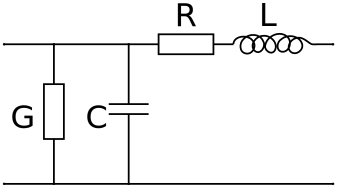
\includegraphics[scale=0.6]{ersatzschaltung}
\label{fig:ersatz}
\caption{%
Ersatzschaltung eines Koaxialkabels zwischen $x$ und $x + \d x$.  Die
Größen $R, L, G, C$ heißen Leitungskonstanten oder Leitungsbeläge.  Bei
einer verlustfreien Leitung ist $R = G = 0$.  Durch eine Betrachtung
dieser Ersatzschaltung kann die Telegraphengleichung hergeleitet
werden.}
\end{figure}

Die Beschreibung der Ausbreitung von Signalen auf Leitungen ist
Gegenstand der Leitungstheorie.  Eine Leitung (zum Beispiel eine
Koaxialleitung, die in diesem Versuch verwendet wird) kann durch zwei
parallel verlaufende Leiter modelliert werden.  Grundaufgabe der
Leitungstheorie ist es, den zeitlichen Verlauf von Stromstärke $I(t, x)$
und Spannung $U(t, x)$ an jedem Ort $x$ der Leitung zu bestimmen.

Dazu wird ein Leitungstück von $x$ nach $x + \d x$ durch die
Ersatzschaltung aus Abbildung~\ref{fig:ersatz} dargestellt.  Die
Leitungsbeläge $R, L, G, C$ heißen auch Leitungskonstanten: $L$
und $C$ heißen Induktivitäts- bzw. Kapazitätsbelag, $R$ und $G$
heißen ohmscher Belag bzw. Querleitfähigkeitsbelag.  Die beiden
letzten kommen durch die endliche Leitfähigkeit des
Leitermaterials (Längsspannungsverluste) und dielektrische
Verlustströme zwischen der Isolierung der beiden Leiter zustande.

\subsection{Telegraphengleichung}

Im allgemeinen ergibt sich durch Betrachtung der Ersatzschaltung
ein System gekoppelter partieller Differentialgln. für $U$ und
$I$.  Im Falle konstanter Beläge kann dieses entkoppelt werden
und es folgt eine verallgemeinerte Wellengleichung:
%
\begin{equation}
\label{eq:wellengl.}
\pdn{2}{U}{x} - LC \pdn{2}{U}{t} = (LG+RC) \pd{U}{t} + RGU
\end{equation}
%
Diese Gleichung wird auch oft als Telegraphengleichung
bezeichnet.  Die Lösungen sind gedämpfte, hin- und rücklaufende
harmonische Wellen:
%
\begin{equation}
\label{eq:loesung}
U(t, x) = U_0 \,e^{\mathrm{i}\omega t \pm \gamma x}
\end{equation}
%
Der Faktor $\gamma = \alpha + \mathrm{i}\beta
= \sqrt{(R+\mathrm{i} \omega L)(G + \mathrm{i} \omega C)}$ heißt
Ausbreitungskonstante, $\alpha$ heißt Dämpfungsbelag und $\beta$
heißt Phasenbelag.  Die Phasengeschwindigkeit der Welle ist daher
frequenzabhängig und führt zu einer Verzerrung des Signals.

\subsection{Leitungswellenwiderstand}

Die Art der Verzerrung wird vom Leitungswellenwiderstand
beeinflußt, welcher durch das Verhältnis von Strom- und
Spannungswellen, die sich in eine gemeinsame Richtung ausbreiten,
bestimmt ist.  Für ein sinusförmiges Signal mit der Frequenz
$\omega$ ist der Wellenwiderstand daher
%
\begin{equation}
\label{eq:wellenwiderstand}
Z_0 = \frac{U(\omega)}{I(\omega)} = \sqrt{\frac{R + \mathrm{i} \omega
L}{G + \mathrm{j} \omega C}}\:.
\end{equation}
%

\subsection{Spannungs- und Strompulse}

In der Digital- und Nachrichtentechnik haben die Signale, die
über eine Leitung übertragen werden, oft die Form eines Pulses.
Die Lösungen der entsprechenden Telegraphengleichung haben dann
die Form eines hin- und rücklaufenden Pulses, der durch die
Reflexion am Leitungsende entsteht.  Der Quotient
%
\begin{equation}
\Gamma = \frac{U_\text{r}}{U_0} = \frac{Z_L - Z_0}{Z_L + Z_0}
\end{equation}
%
heißt Reflexionsfaktor.  Mit seiner Hilfe kann die Form der
rücklaufenden Welle aus dem Eingangspuls berechnet werden.  Dazu
wird die \name{Laplace}-Transformation verwendet.  Sei nämlich
$\tilde{U}_0(s)$ die \name{Laplace}-Transformierte der Spannung
des einlaufenden und $\tilde{U}_\text{r}(s)$
die \name{Laplace}-Transformierte der Spannung des reflektierten
Signals am Ort $x$ zur Zeit $t$, dann gilt
%
\begin{equation}
\tilde{U}_\text{r}(s) = \Gamma\, \tilde{U}_0(s).
\end{equation}
%
Aus der Umkehrung dieser Formel unter Ausnutzung der
inversen \name{Laplace}-Transformation der zeitliche Verlauf der
Spannung $U_\text{r}(t, x)$ bestimmt werden.

\section{Durchführung}

\end{document}
